\documentclass[tikz]{standalone}

\usetikzlibrary{calc,decorations.markings}
\usepackage{amsfonts,amsmath,amsthm,amssymb,mathtools,stmaryrd,mathrsfs}

\begin{document}
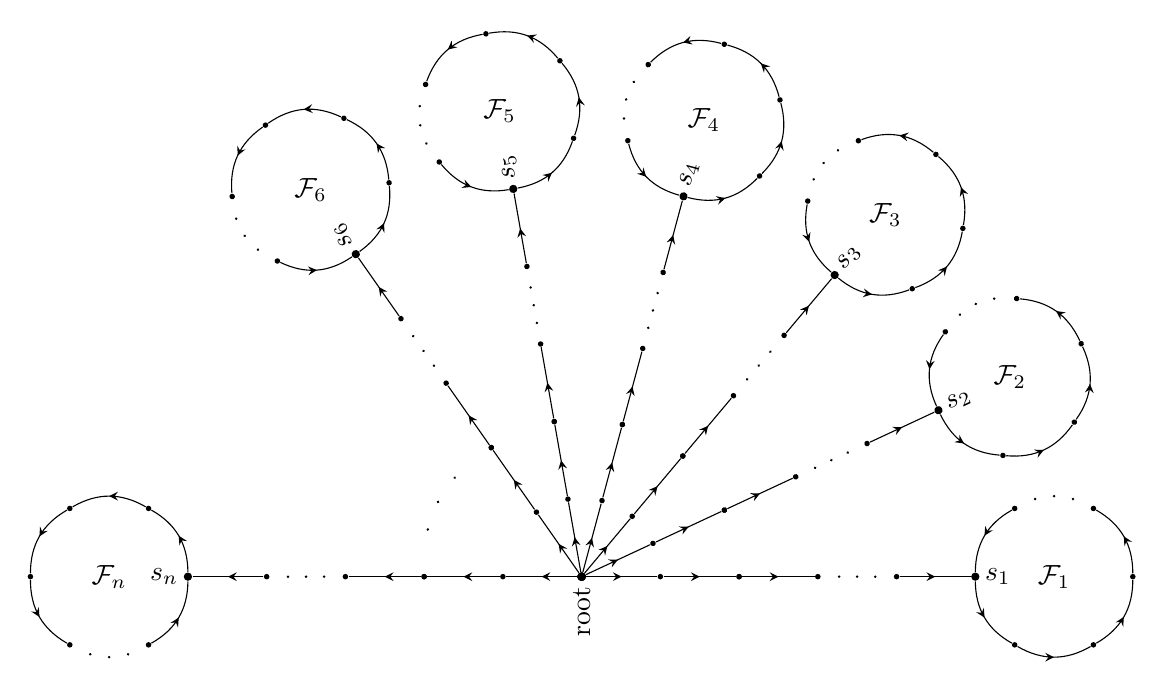
\begin{tikzpicture}[>=stealth,
	]

	\tikzset{middle arrow/.style={
				postaction=decorate,
				decoration={
						markings,
						mark=at position 0.5 with {\arrow{>}}}}
	}
	\tikzset{dotted pattern/.style={
				postaction=decorate,
				decoration={
						markings,
						mark=
						between positions 0.25 and 0.75 step 0.25
						with
							{
								\fill[radius=0.5pt,black] (0,0) circle;
							}
					}
			}
	}
	\tikzset{dotted pattern2/.style={
				postaction=decorate,
				decoration={
						markings,
						mark=
						between positions 0.3 and 0.7 step 0.2
						with
							{
								\fill[radius=0.5pt,black] (0,0) circle;
							}
					}
			}
	}

	\node[circle,fill=black,inner sep=0pt,minimum size=3pt] (root) at (0,0){} node[left,rotate=90]{root};

	\def\InnerScope{
		\node[circle,fill=black,inner sep=0pt,minimum size=3pt] (root) at (0,0){};

		\node [circle,fill=black,inner sep=0pt,minimum size=2pt] (n1) at (1,0) {};
		\draw[middle arrow] (root) --%node[above=-1pt]{\small $p_{\i,1}$}
		(n1);

		% this is a node that will be used later
		\node [circle,fill=black,inner sep=0pt,minimum size=2pt] (X\i) at (2,0) {};

		\node [circle,fill=black,inner sep=0pt,minimum size=2pt] (n2) at (2,0) {};
		\draw[middle arrow] (n1) --%node[above=-1pt]{\small $p_{\i,2}$} 
		(n2);

		\node [circle,fill=black,inner sep=0pt,minimum size=2pt] (n3) at (3,0) {};
		\draw[middle arrow] (n2) --%node[above=-1pt]{\small $p_{\i,3}$} 
		(n3);

		\node [circle,fill=black,inner sep=0pt,minimum size=2pt] (n4) at (4,0) {};
		% \node [] (path_cdots) at (3.5,0) {$\cdots$};
		\draw[draw=none,dotted pattern] (n3) --%node[above=-1pt]{\small $p_{\i,3}$} 
		(n4);

		\node [circle,fill=black,inner sep=0pt,minimum size=3pt] (n5) at (5,0) {};
		% \draw[middle arrow] (n4) --%node[above=-1pt]{\small $p_{\i,k_\i}$} 
		% (n5) node[right]{$s_\i$};


		\node [circle,fill=black,inner sep=0pt,minimum size=2pt] (m1) at ($(5,0) + (1,0) + ({cos(180 + 60)},{sin(180 + 60)})$) {};
		\draw[middle arrow] (n5) to [bend right] %node[left=-1pt]{\small $c_{\i,1}$} 
		(m1);

		\node [circle,fill=black,inner sep=0pt,minimum size=2pt] (m2) at ($(5,0) + (1,0) + ({cos(180 + 60*2)},{sin(180 + 60*2)})$) {};
		\draw[middle arrow] (m1) to [bend right] %node[below=-1pt]{\small $c_{\i,2}$} 
		(m2);

		\node [circle,fill=black,inner sep=0pt,minimum size=2pt] (m3) at ($(5,0) + (1,0) + ({cos(180 + 60*3)},{sin(180 + 60*3)})$) {};
		\draw[middle arrow] (m2) to [bend right] %node[right=-1pt]{\small $c_{\i,3}$} 
		(m3);

		\node [circle,fill=black,inner sep=0pt,minimum size=2pt] (m4) at ($(5,0) + (1,0) + ({cos(180 + 60*4)},{sin(180 + 60*4)})$) {};
		\draw[middle arrow] (m3) to [bend right] %node[right=-1pt]{\small $c_{\i, 4}$} 
		(m4);

		\node [circle,fill=black,inner sep=0pt,minimum size=2pt] (m5) at ($(5,0) + (1,0) + ({cos(180 + 60*5)},{sin(180 + 60*5)})$) {};
		\draw [draw=none,dotted pattern] (m4) to [bend right] (m5);

		\draw[middle arrow] (m5) to [bend right] %node[left=-1pt]{\small $c_{\i,\ell}$} 
		(n5);
	}


	\foreach \i/\angle in {1/0, 2/25, 3/50, 4/75, 5/100, 6/125} {

			\begin{scope}[rotate=\angle,every node/.append style={transform shape}]
				\InnerScope
		
        \draw[middle arrow] (n4) --(n5) node[right]{$s_\i$};
			\end{scope}
			\begin{scope}[rotate=\angle]
				\node[] (text) at (6,0) {$\mathcal F_\i$};
			\end{scope}

		}

		{
			\def\i{n}
			\def\angle{180}

			\begin{scope}[rotate=\angle]
				\InnerScope
        \draw[middle arrow] (n4) --(n5) node[left]{$s_\i$};
				\node[] (text) at (6,0) {$\mathcal F_\i$};
			\end{scope}

		}

	\draw [draw=none,dotted pattern2] (X6) to [bend right] (Xn);

\end{tikzpicture}
\end{document}
